\section{Schedules}

  We have two pipelines, the \textbf{\textit{catalogue}} pipeline that is responsible for all the data that is currently accessible to partners on iPlayer
  and the new \textbf{\textit{schedules}} pipeline. We first have to ingest the schedule data from another source, which consists of over 1000 files and 
  then parse that data for what we want to share with partners. This parsed data is then stored in redis for future use. In the older catalogue pipeline 
  this process was done by an EC2 (server), however with this pipeline we wanted less to manage and decided to go with a lambda (serverless) approach. To speed 
  up ingestion of data we decided to experiment with multiple lambdas being invoked at the same time for concurrent processing of the files. 
  This is the part of the project I was tasked to document/create.
  
  \begin{figure}[H]
    \centering
    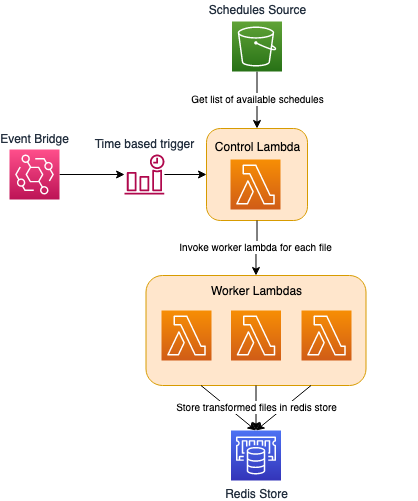
\includegraphics[width=6cm]{assets/ingester.drawio.png}
    \caption{Ingester AWS architecture.}
    \label{fig:ingesterArch}
  \end{figure}

  Figure 4 shows what the cloud infrastructure on AWS looks like. We get an event from event bridge, the available data is then retrieved from source and the
  parsing is then handed over to multiple concurrent lambdas. Finally this data is stored in redis for the next component in the pipeline to use. I have 
  illustrated this flow in the sequence diagram below.

  \begin{figure}[H]
    \centering
    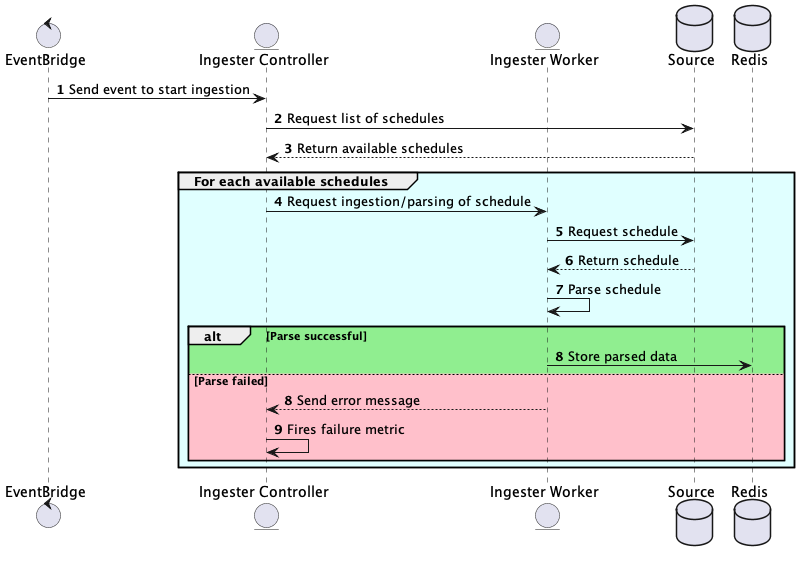
\includegraphics[width=8cm]{assets/diagrams/ingesterBasicFlow.png}
    \caption{Ingester basic execution sequence diagram.}
    \label{fig:ingesterFlow}
  \end{figure}

  For completeness I have also drawn a sequence diagram for the removal of old schedules from the redis store. This process is done just before the 
  parallelised lambdas are called to do their work. Removal is important here as if they were not removed it would have a knock on effect down the pipeline 
  as there would be unnecessary processing done for schedules that are no longer being used or accessible to partners.

  \begin{figure}[H]
    \centering
    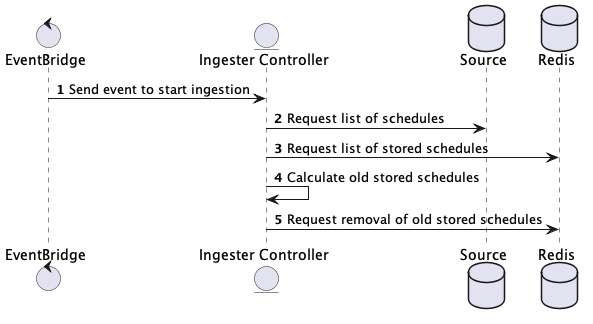
\includegraphics[width=8cm]{assets/diagrams/ingesterDataRemoval.png}
    \caption{Ingester old data removal sequence diagram.}
    \label{fig:ingesterScheduleRemoval}
  \end{figure}

  In the pipeline there is a second component called the \textit{Schedule Generator} that is responsible for outputting the data in a format partners will
  receive. For this component we did not have the worker lambda, and instead had a single lambda do all the processing. The two graphs belows show the 
  difference in lambda runtime between the two components.

  \begin{figure}[H]
    \centering
    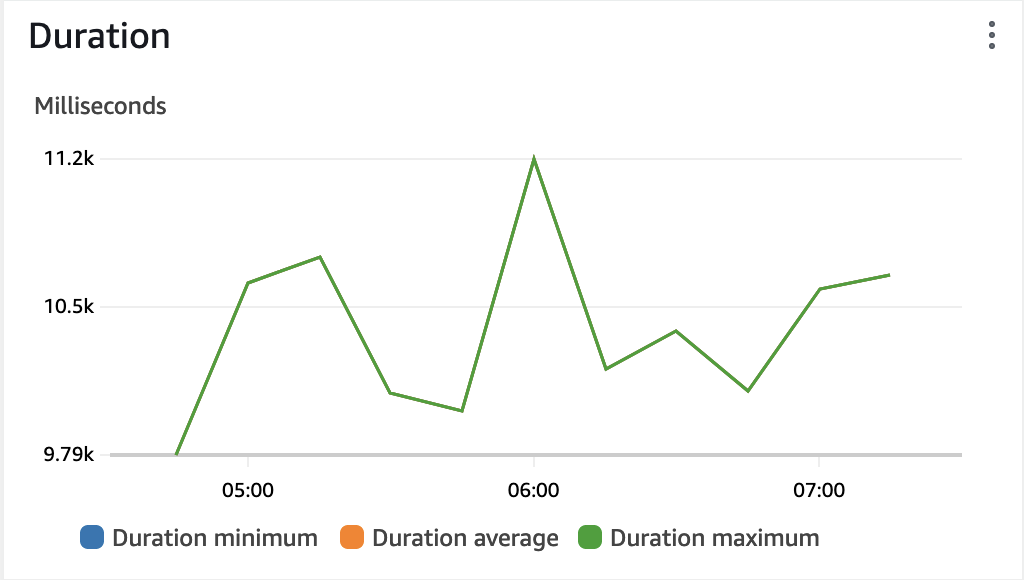
\includegraphics[width=6cm]{assets/ingesterDuration.png}
    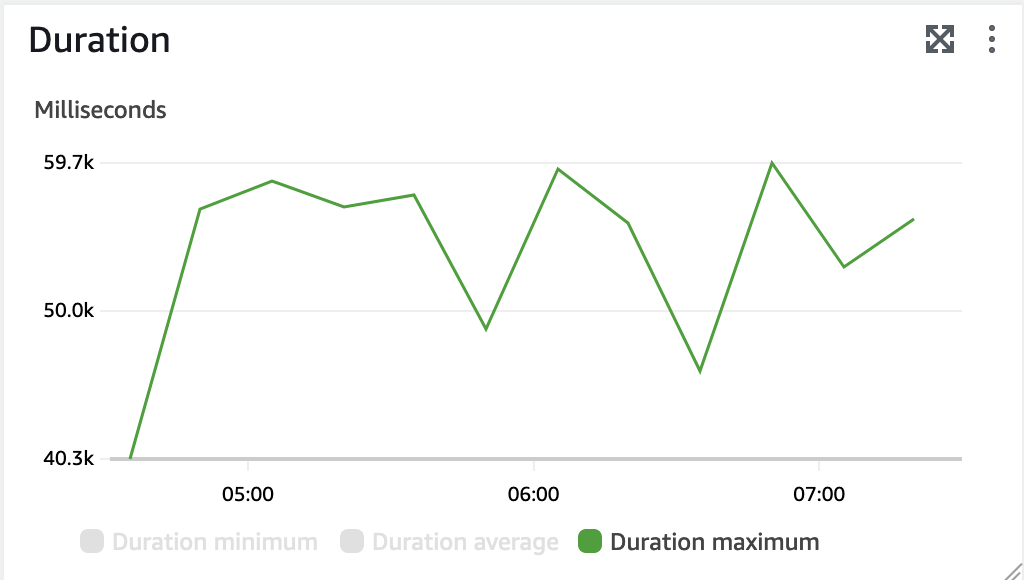
\includegraphics[width=6cm]{assets/generatorDuration.png}
    \caption{Screenshot of AWS lambda duration for schedule Ingester (left) and Generator (right).}
    \label{fig:lambdaDurationDifference}
  \end{figure}

  As can be seen, using parallelised lambdas is 4x quicker on average than using a single lambda. This is important as the quicker this pipeline can run
  the 'fresher' the data is for partners. After seeing these results there is now some talks about also changing the Schedule Generator to use the same 
  pattern.

  \vspace{0.2cm}

  This was also the first project where we upgraded to using the new version of the AWS SDK. This was something we hadn't looked into however was something
  that would be beneficial when we had to upgrade to node 18. AWS would no longer package version 2 of their SDK by default in lambdas. This would result in
  \todo[noline, size=\small]{L3, T2}
  an extra ~70MB of unpacked data being added to the final build which would slow down our build time and cost us a little bit more money, albeit fractions of
  a penny. I lead the investigation into using the new SDK and if it was feasible. This upgrade then also lead to the upgrade of our credentials provider
  which had security vulnerabilities that needed fixing.

  \begin{figure}[H]
    \centering
    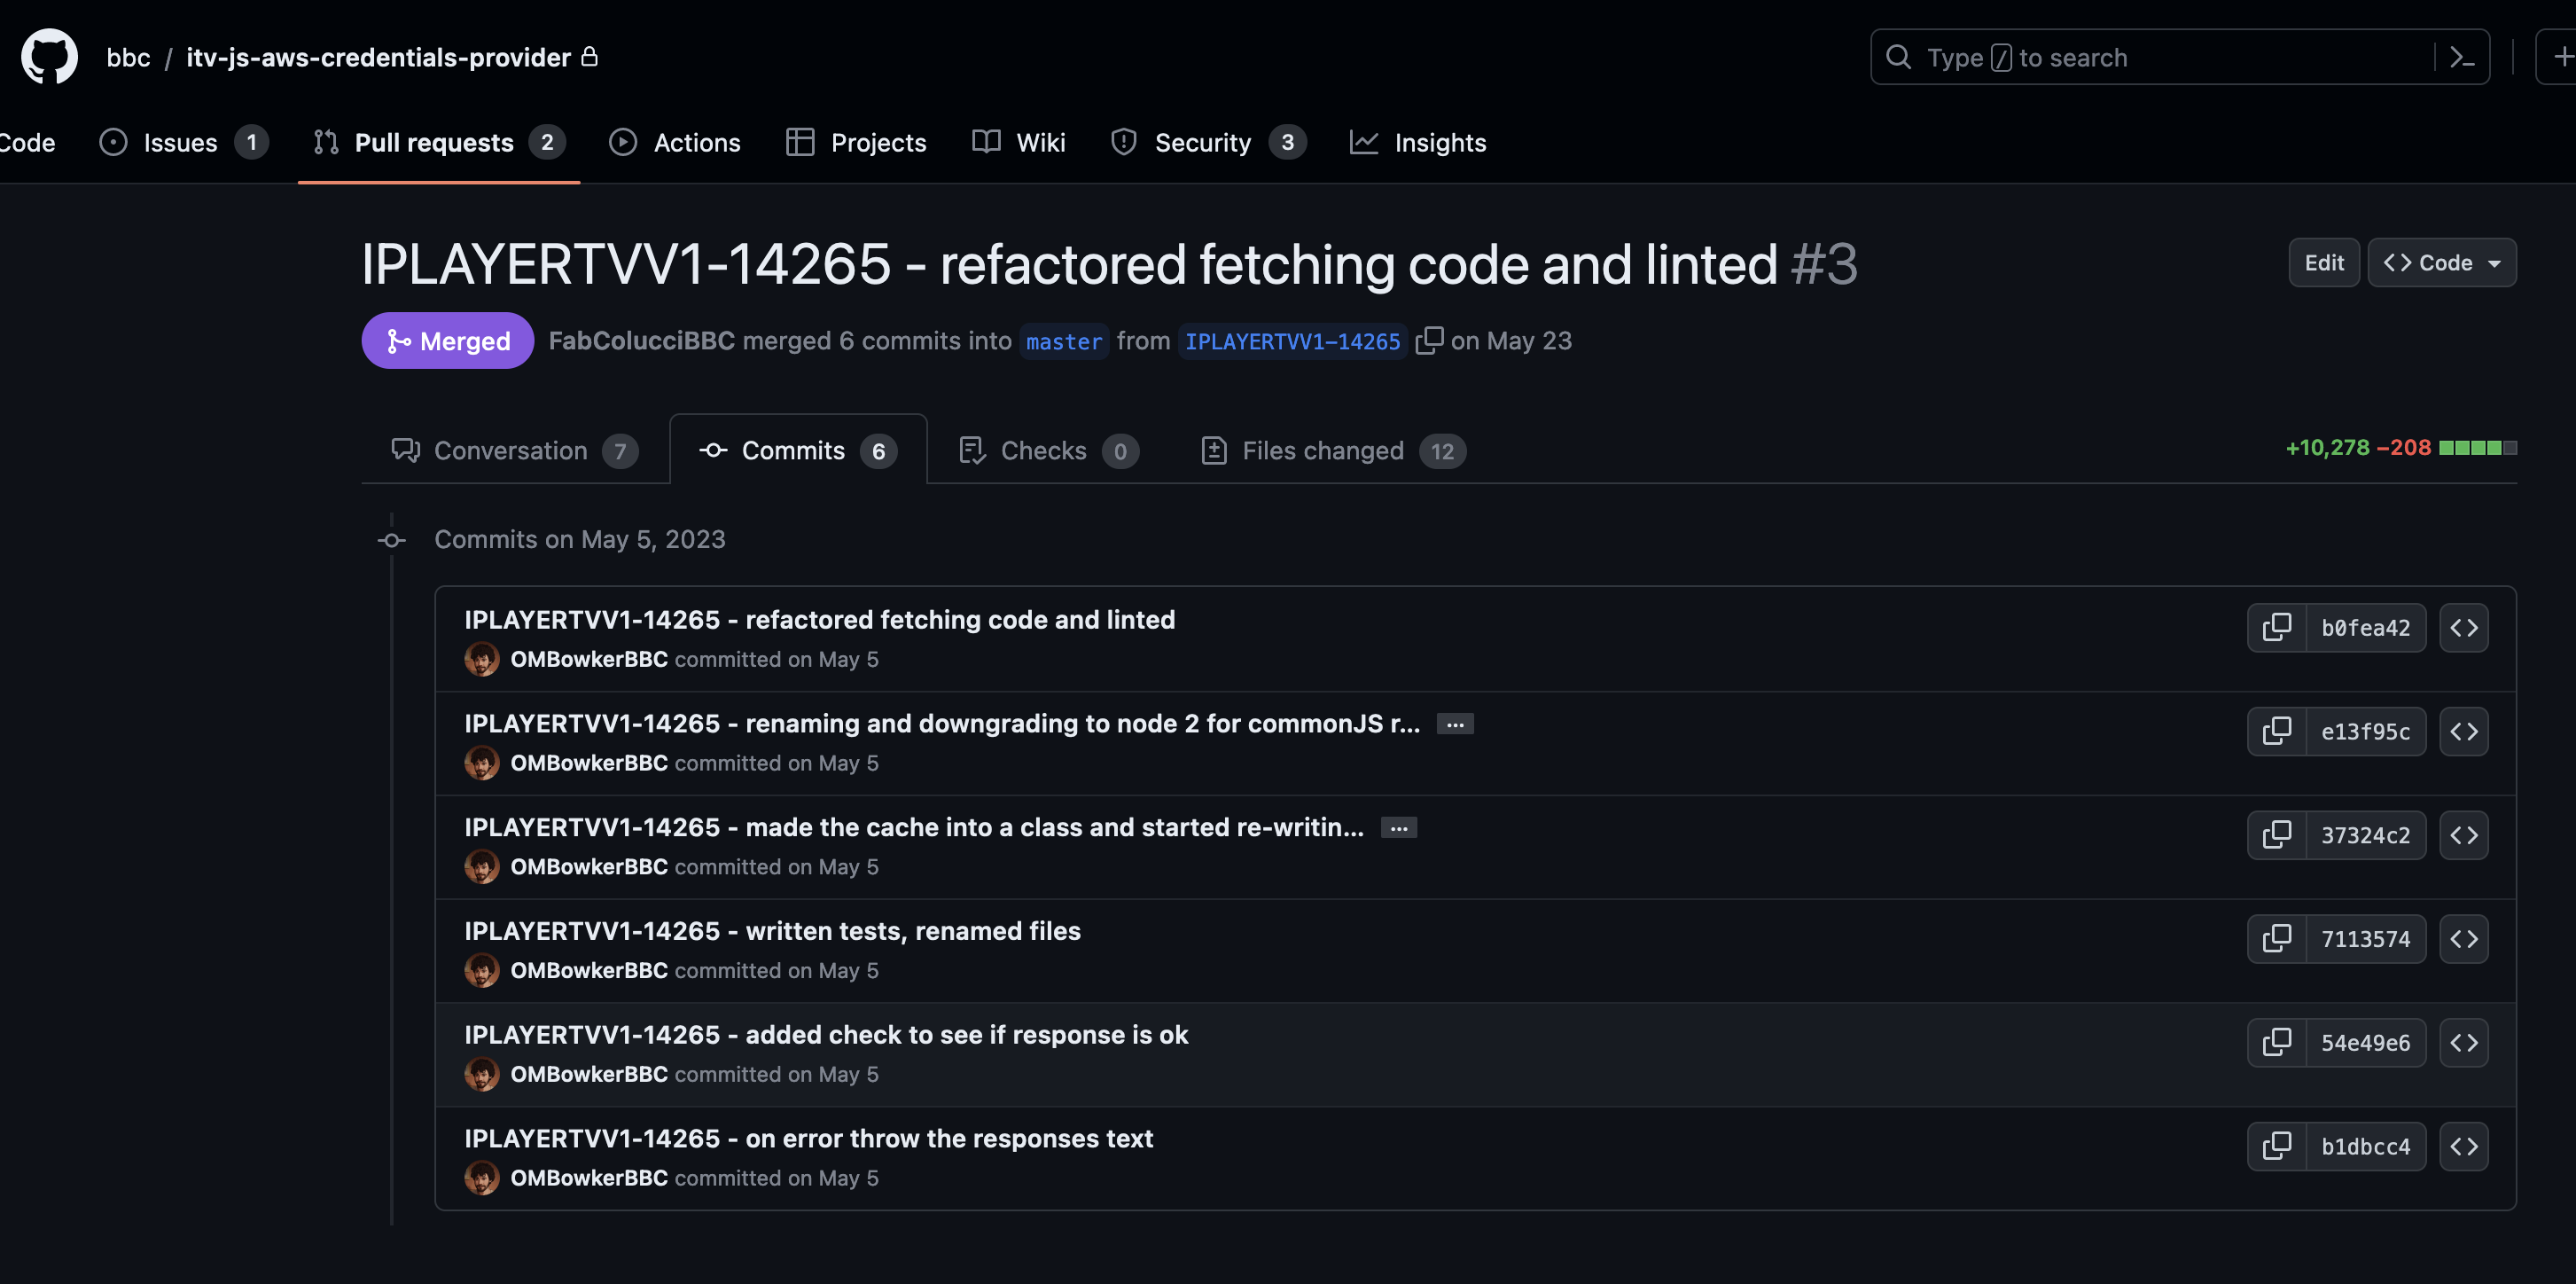
\includegraphics[width=6cm]{assets/credentialsRefactorCommits.png}
    \caption{Screenshot commits for credentials refactor.}
    \label{fig:credentialsRefactor}
  \end{figure}

  \subsection{The reason for schedules}
  Schedules is part of a much larger BBC wide objective to deprecate an external service called Nitro. The deadline for this is October with 
  schedules at the being retrieved from the service that wants to be deprecated. This switch to an internal system will give the BBC more 
  control/oversight of the data, directly contribute to one of our OKRs, (Simplifying Platform), these can be seen in \textbf{ContextSetting.pptx}, 
  and will also save us money in the long run.

  \todo[noline, size=\small]{B6}

  Previously partners were getting there data from this data source, but can now get the same, or even more rich data, from us directly. This can 
  help us with other OKR, like \textit{'Improve our data capabilities'} as it is much easier to track and analyse data that is requested from our 
  own service.

  \subsection{Burn-up charts and planning}
  \todo[noline, size=\small]{B2, P1, T5}
  As schedules was a time sensitive project, it was important that we stayed on track with our work. To help with this our delivery manager 
  used some tools/techniques to visualise and clarify where we were at in development, but also what was to come next. Below is our roadmap
  for the schedules work.

  \begin{figure}[H]
    \centering
    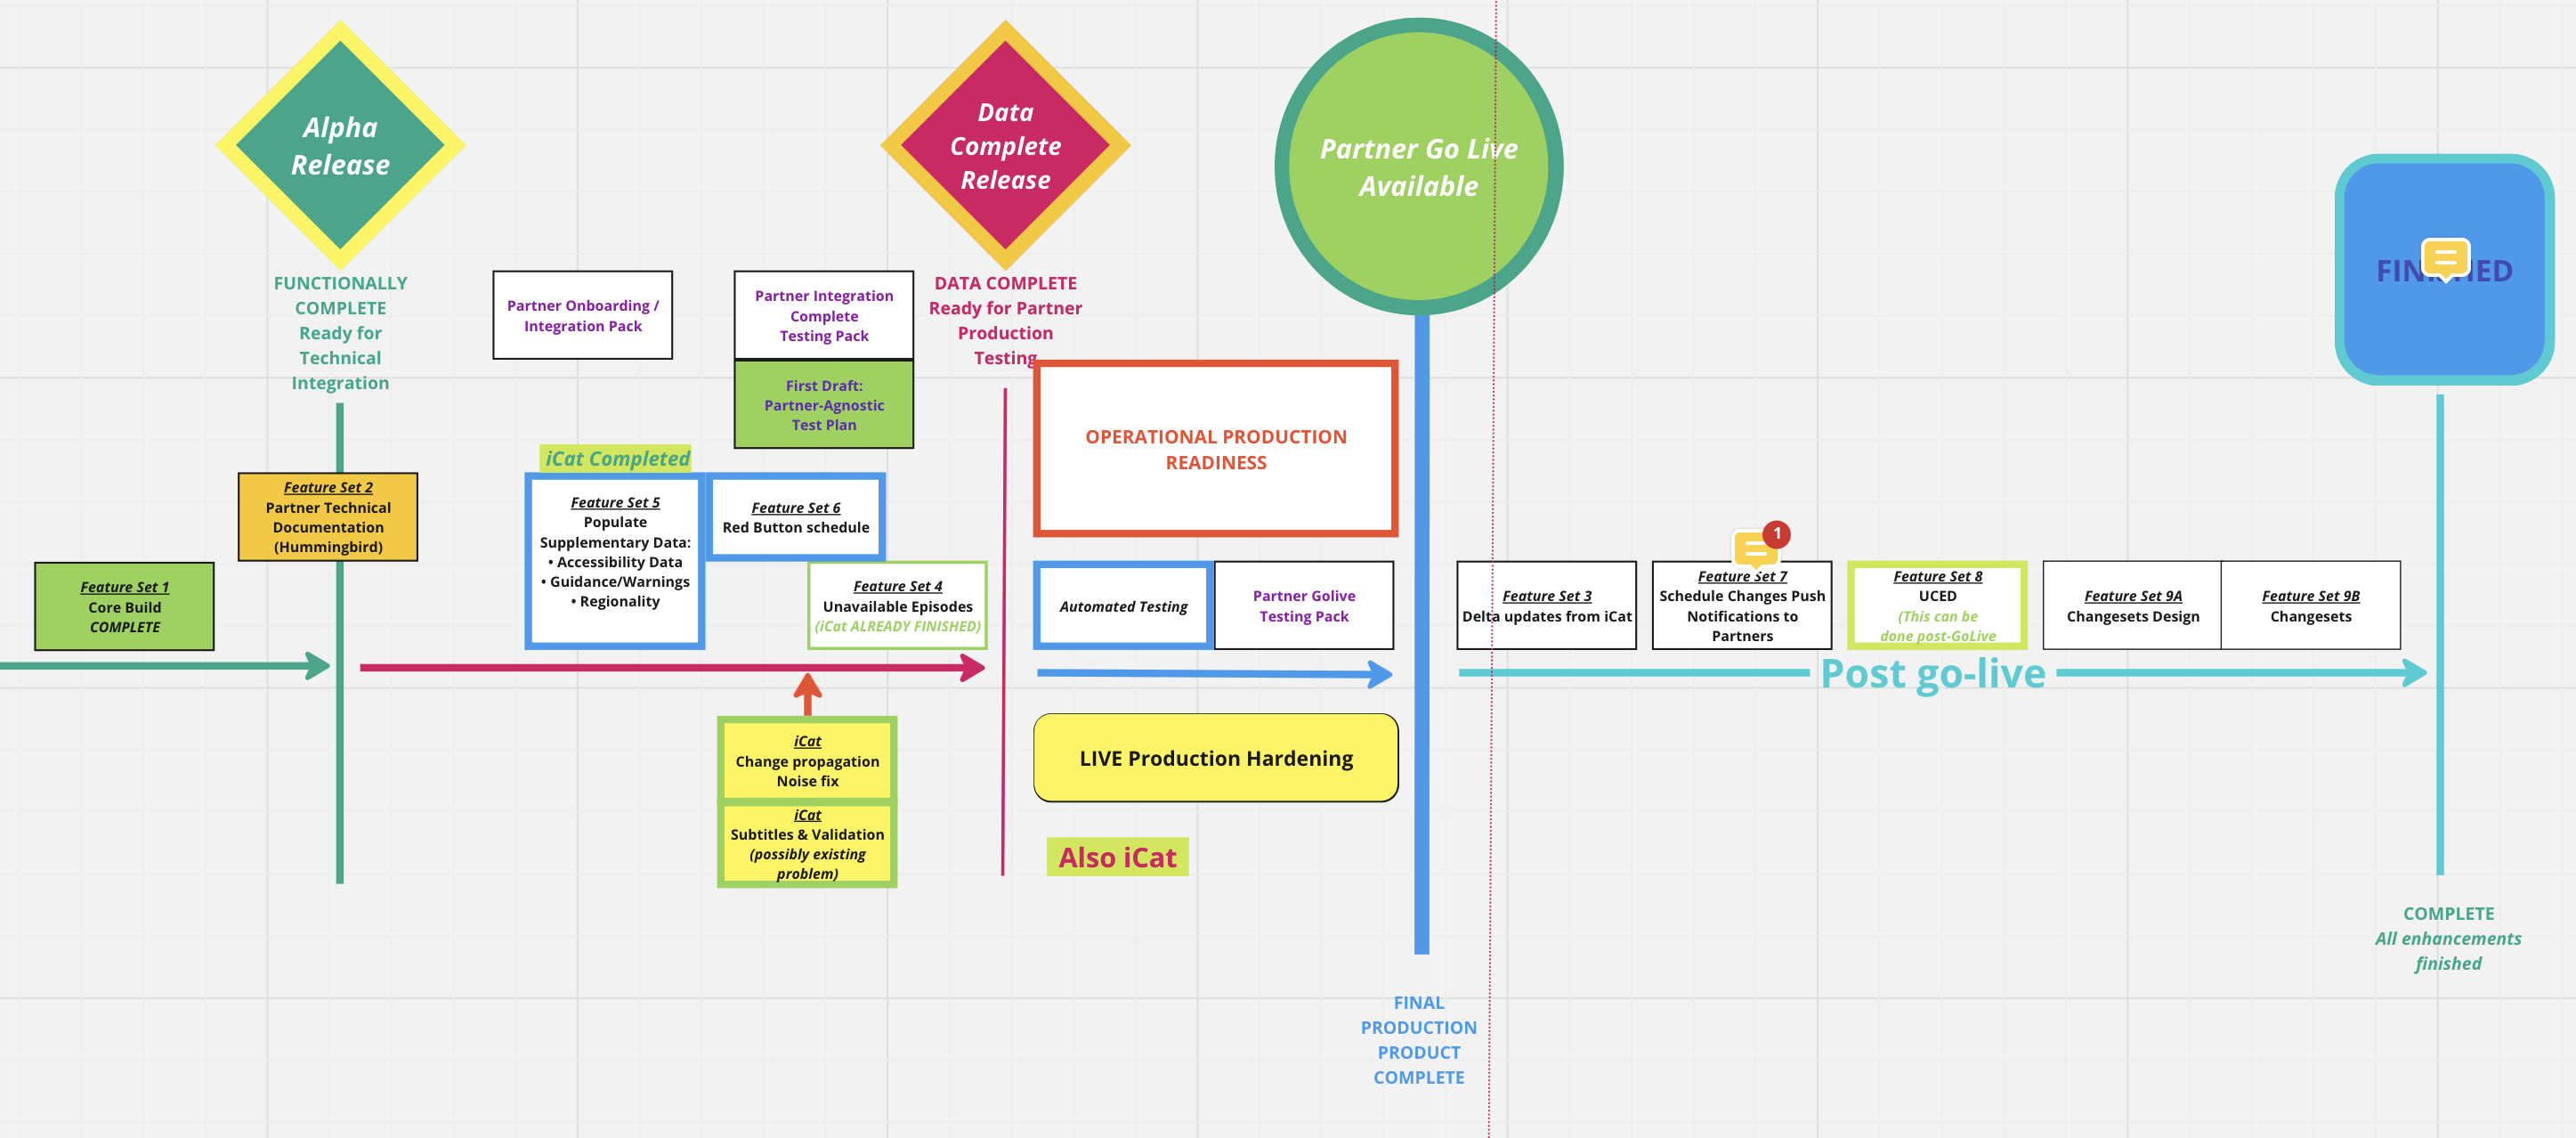
\includegraphics[width=10cm]{assets/schedulesRoadmap.png}
    \caption{Roadmap for schedules.}
    \label{fig:schedulesRoadmap}
  \end{figure}

  We have 4 stages \textit{'Alpha'}, \textit{'Data Complete Release'}, \textit{'Partner Go Live Available'} and \textit{'Finished'}.
  As of writing this we have completed the third stage, meaning that partners are now integrating and using the service. During the 
  creation of this there were many discussion of what needed to be done before each stage was complete.

  An example of this was the creation of automated tests, which would help validate our pipeline was parsing and sending the data to partners correctly.
  This was pushed back to just before partners could go live, but partners would already have access to the information for testing 
  on their systems. This was done as integration can take a long time, with a deadline of October it was vital that partners could start
  working with the data as fast as possible, however we felt that before we could go live we needed the assurance the automated 
  tests would provide us.

  Another discussion was around \textit{'deltas'}, which provide real time updates to the data, instead of a periodic update (every
  15 minutes). After some investigation and discussions it was decided that this was not needed to go live and could be added after, this due again 
  to time constraints but also the relevance of the changes would not be that impactful that the partner needed immediate updates.

  \vspace{0.2cm}

  In addition to roadmapping our delivery manager also used burn-up charts throughout the development of the project. Atlassian describes a
  burn-up chart as:

  \begin{quote}
    \textit{'The Burnup Chart provides a visual representation of a sprint's completed work compared with its total scope. It offers insights 
    on your project's progress, as well as offers warnings to help you maintain your project's health; you can instantly identify problems such 
    as scope creep or a deviation from the planned project path.'} [TODO1]
  \end{quote}

  The burn-up charts can be seen in the following images.
  
  \begin{figure}[H]
    \centering
    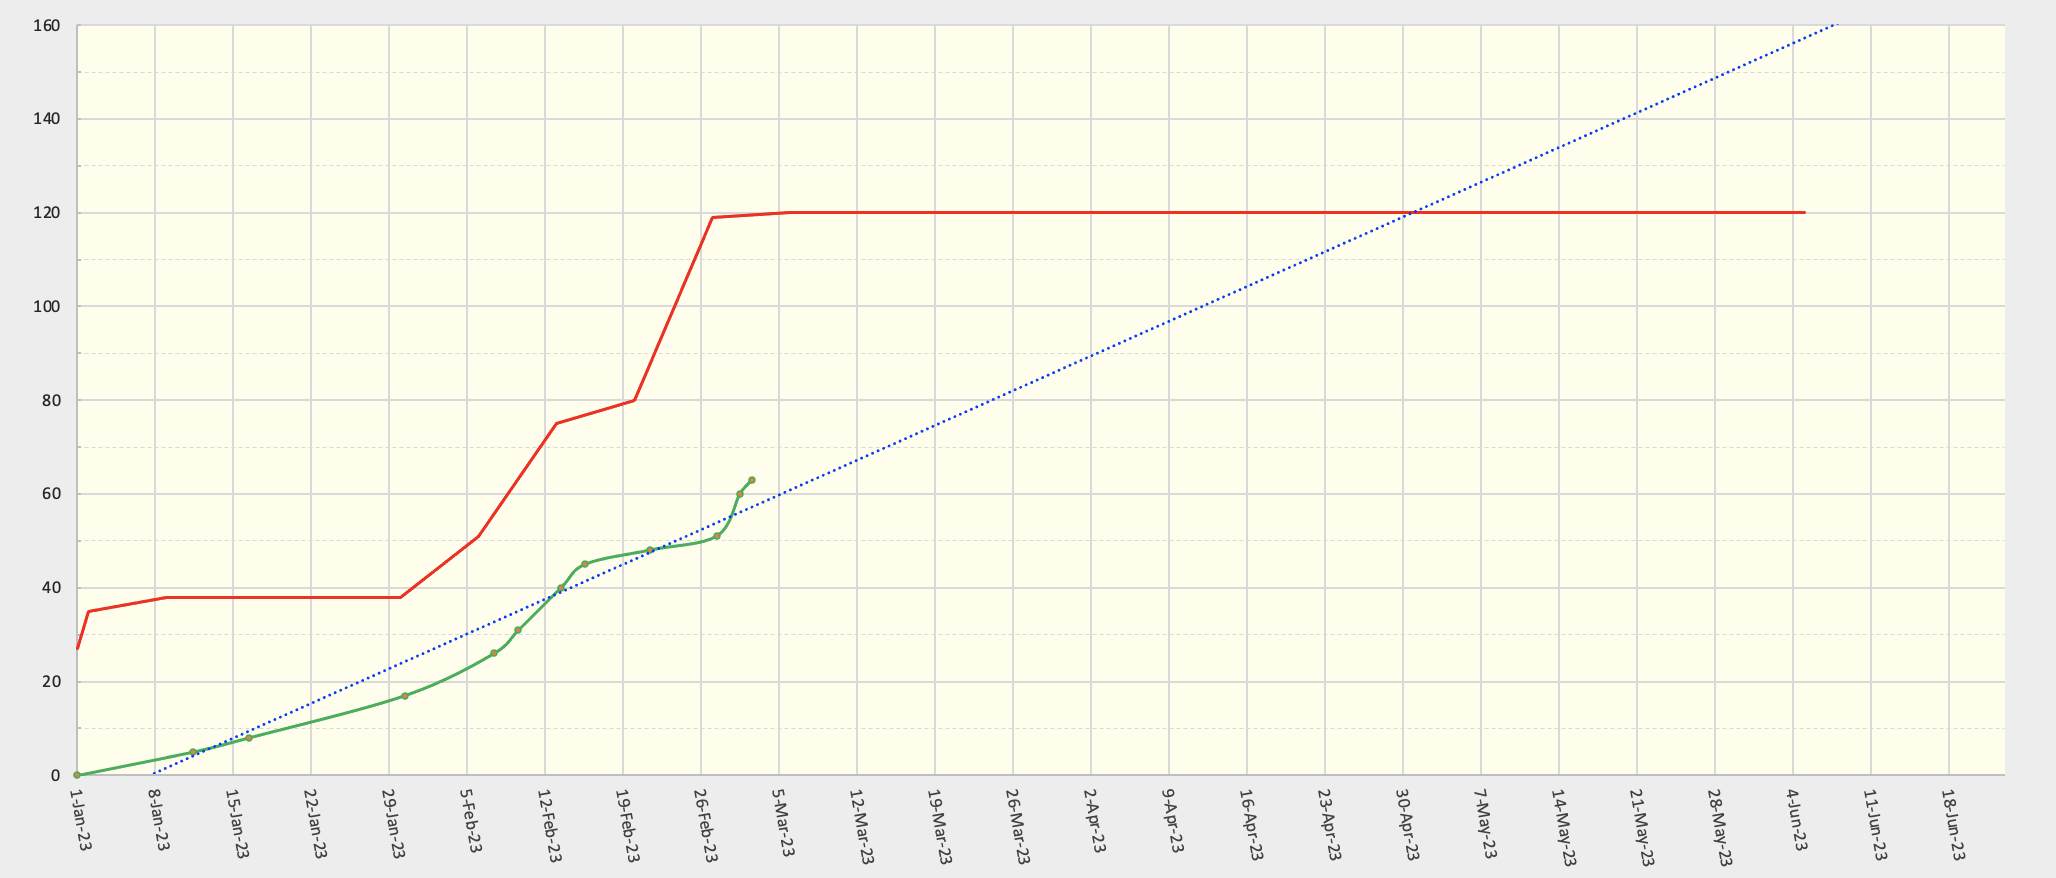
\includegraphics[width=6cm]{assets/burnup/2023-03-03.png}
    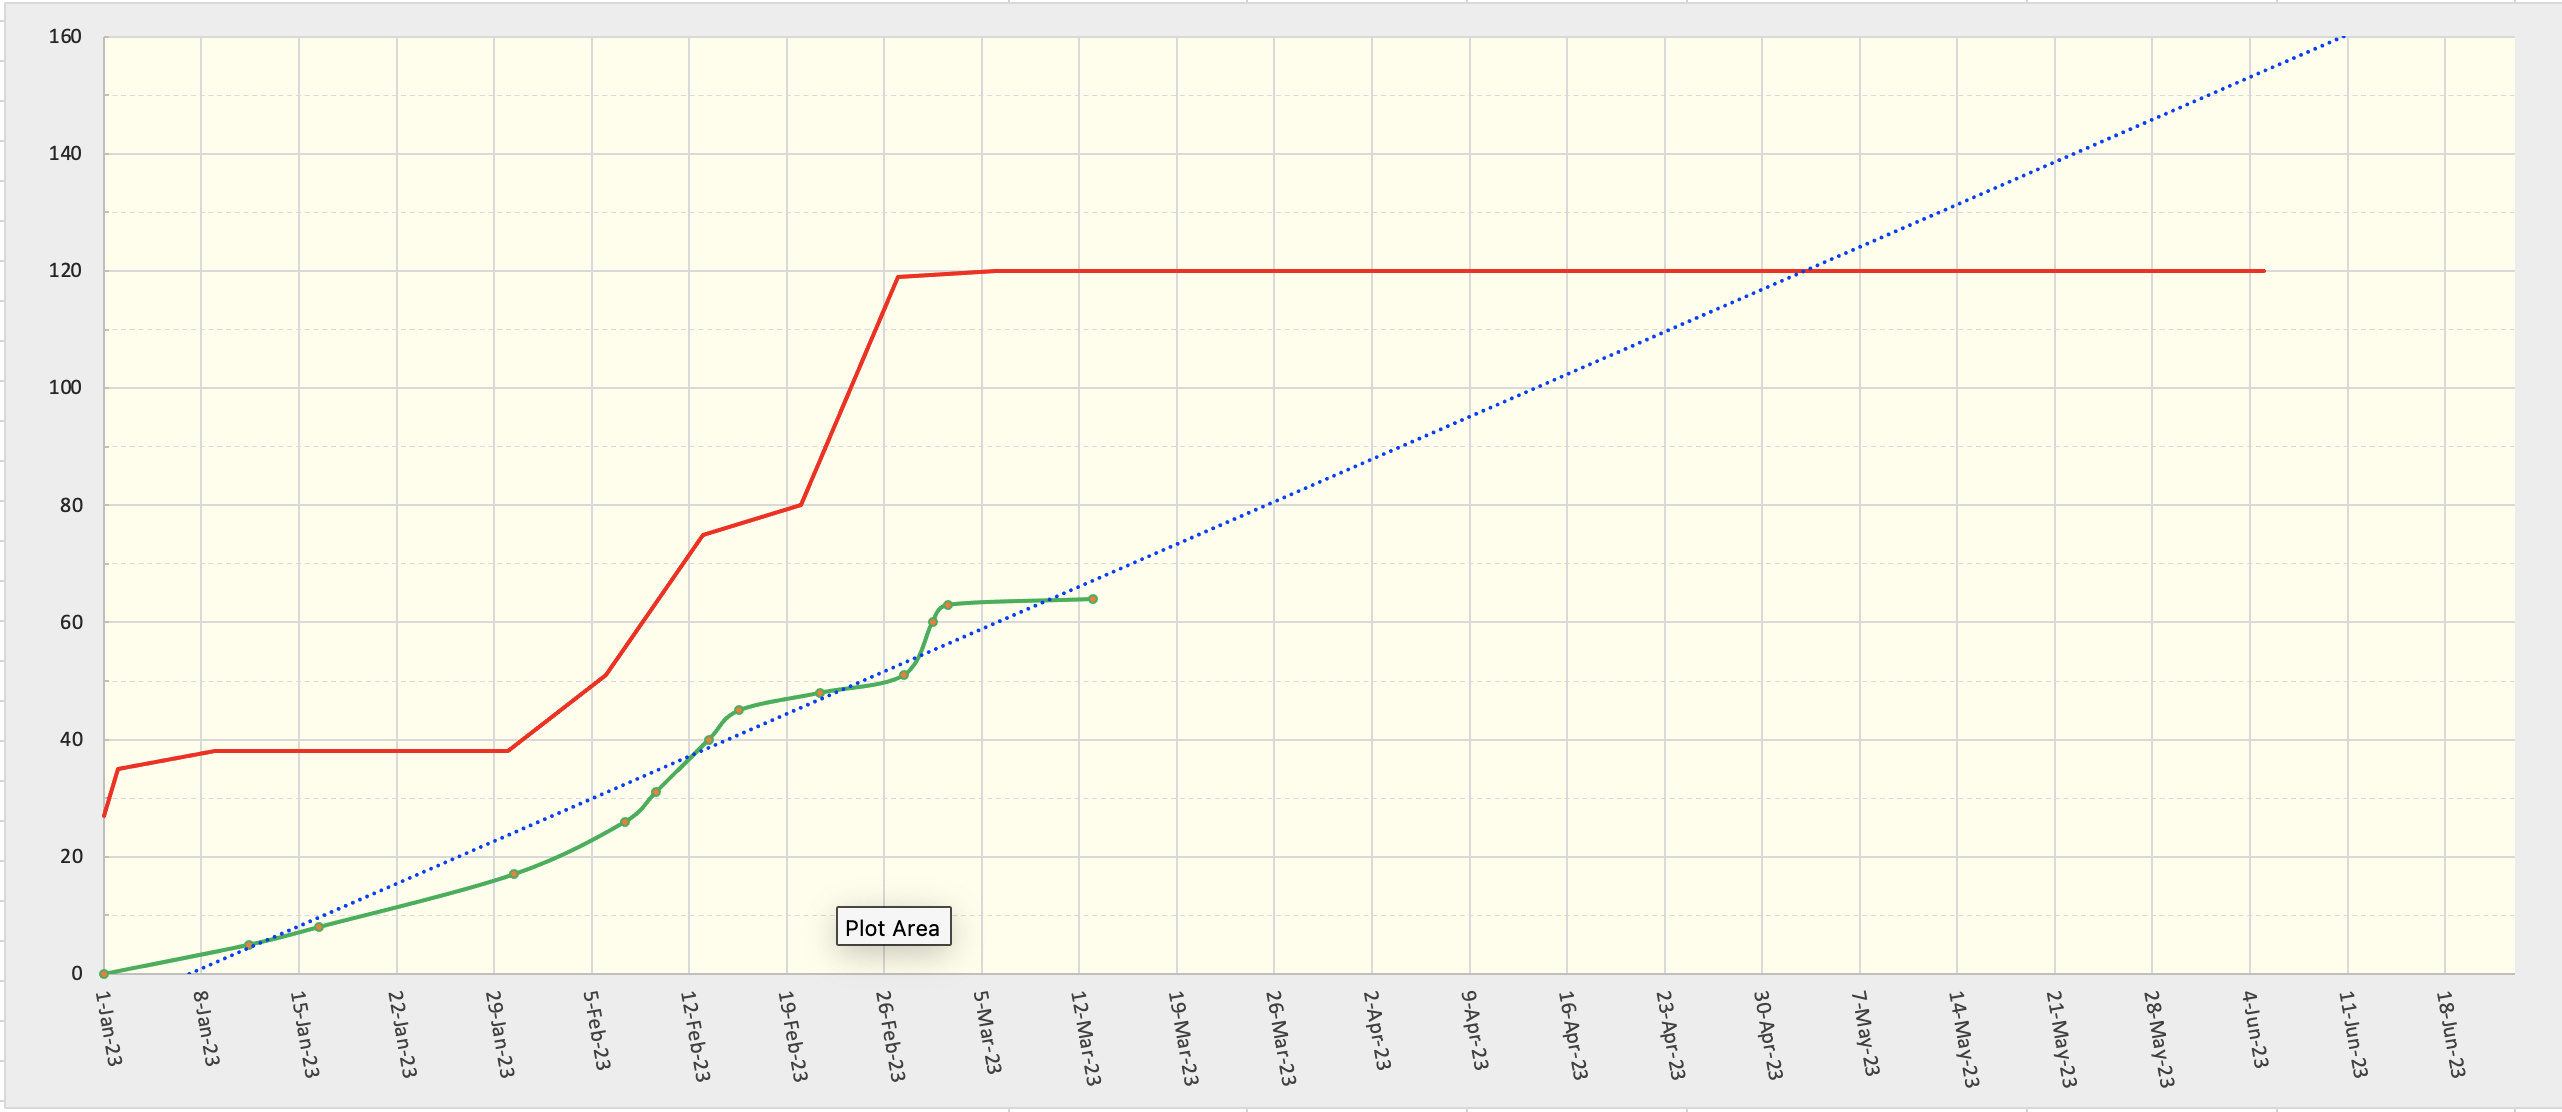
\includegraphics[width=6cm]{assets/burnup/2023-03-14.png}
    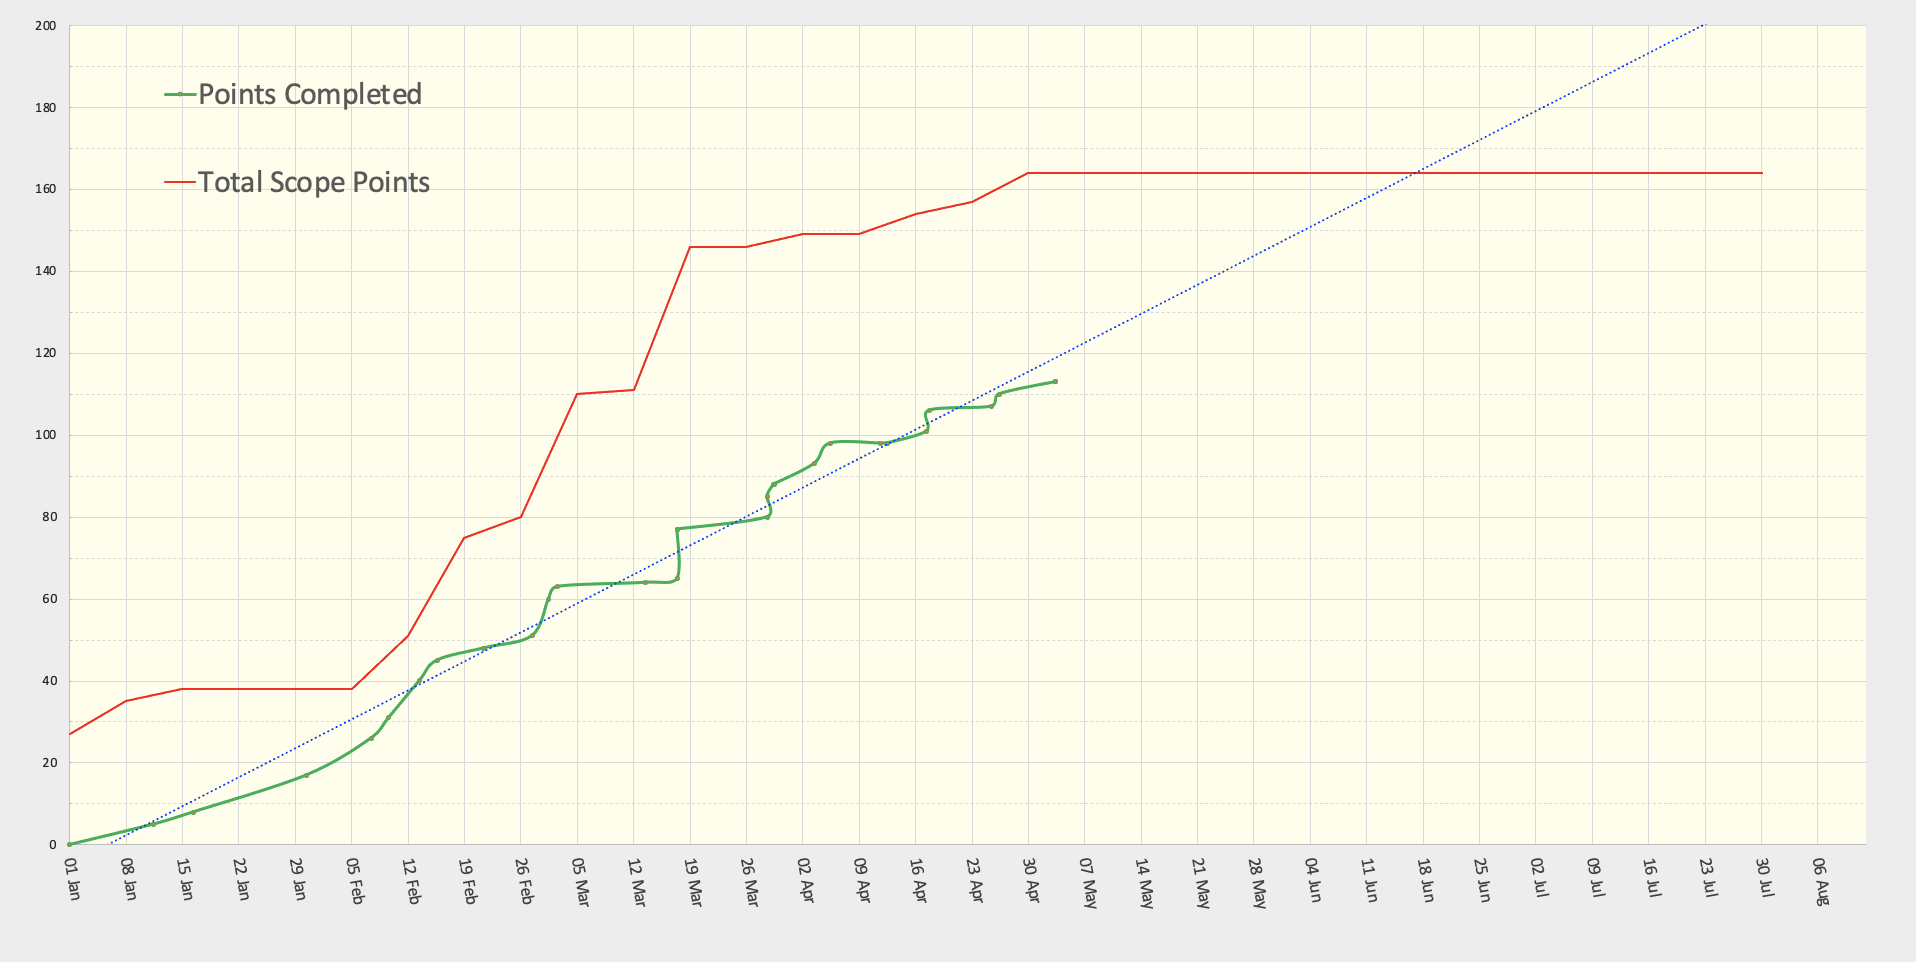
\includegraphics[width=6cm]{assets/burnup/2023-05-03.png}
    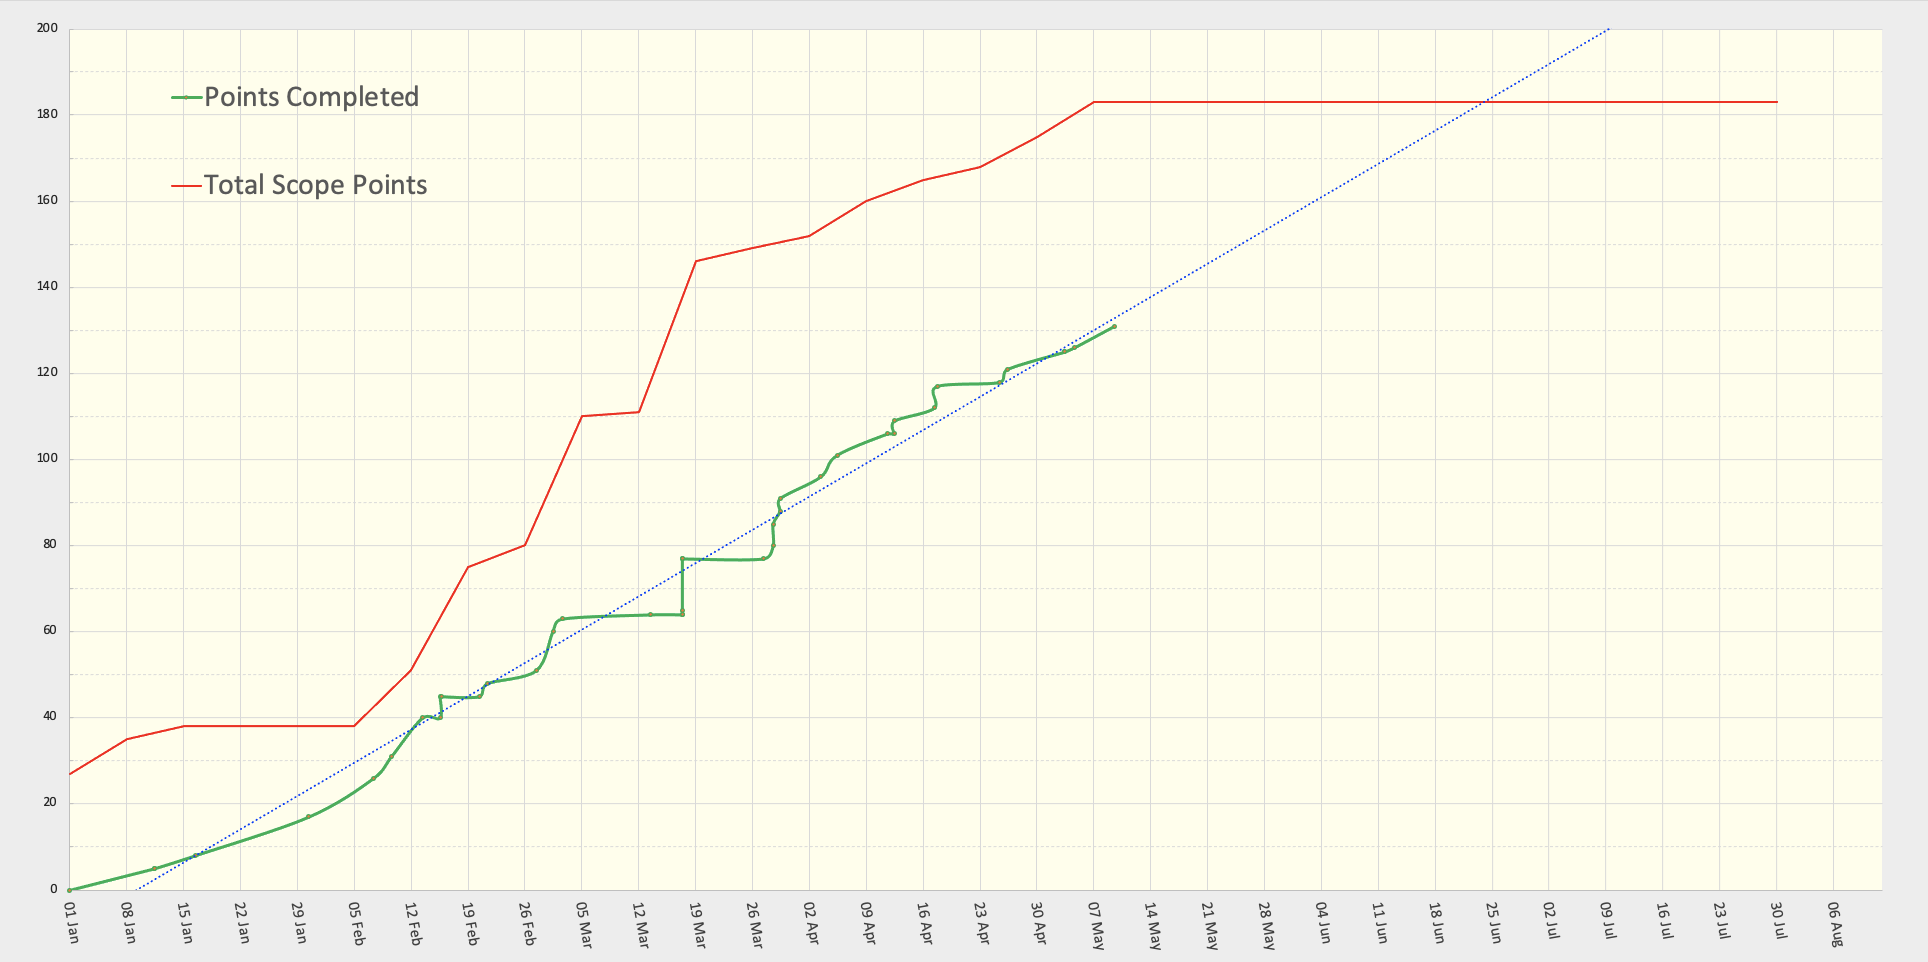
\includegraphics[width=6cm]{assets/burnup/2023-05-10.png}
    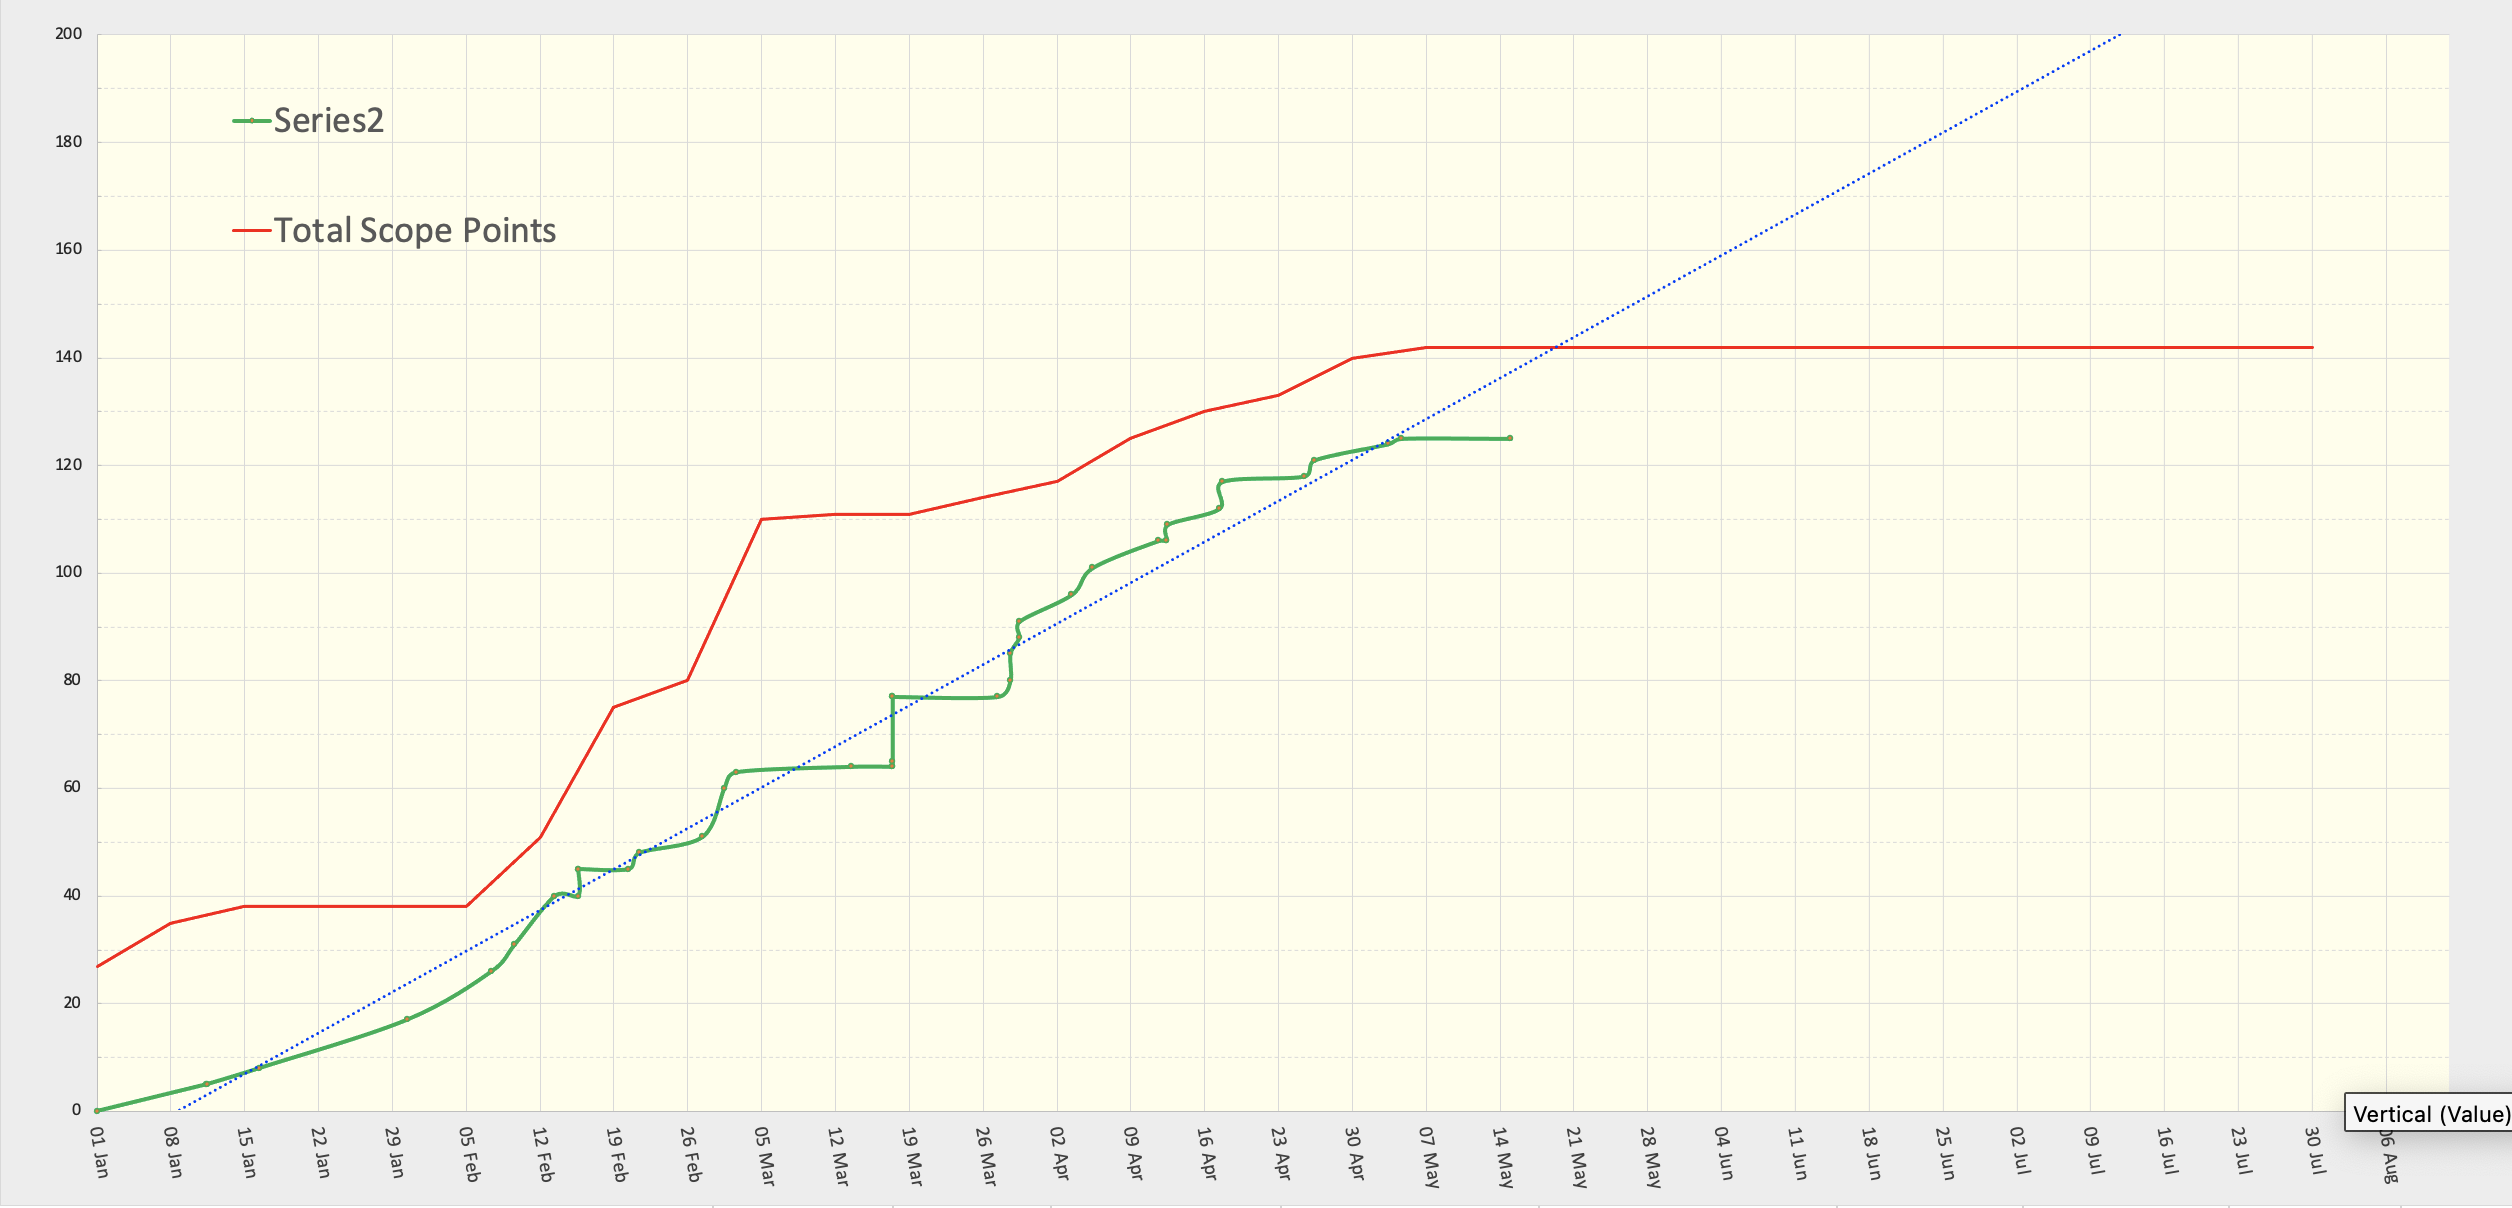
\includegraphics[width=6cm]{assets/burnup/2023-05-15.png}
    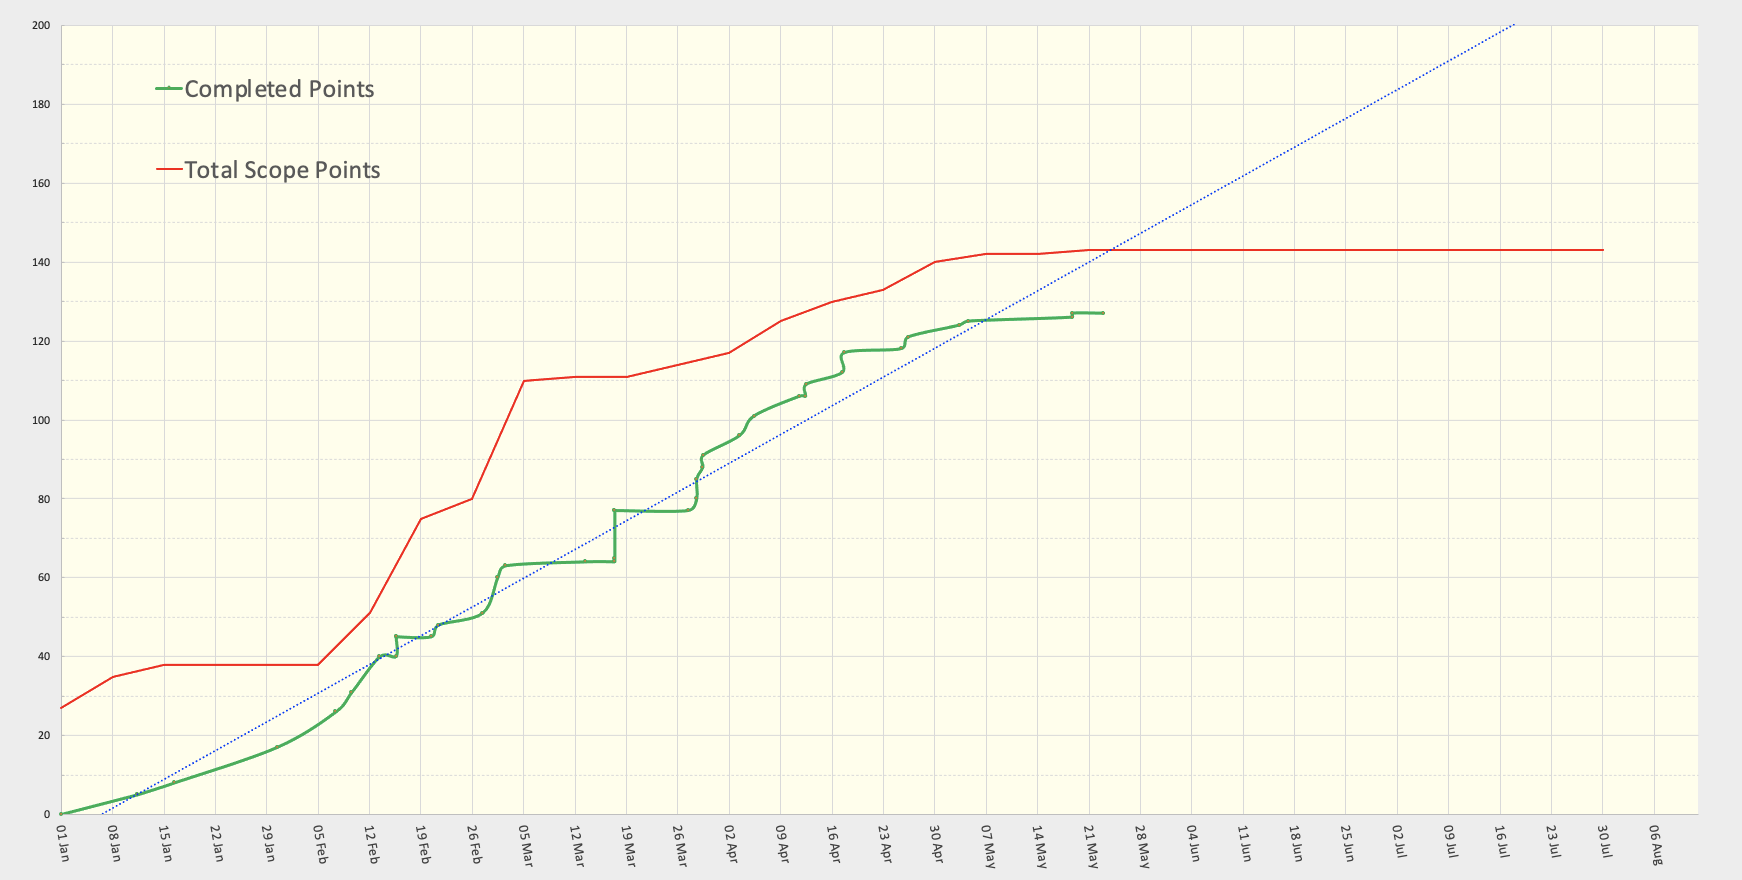
\includegraphics[width=6cm]{assets/burnup/2023-05-23.png}
    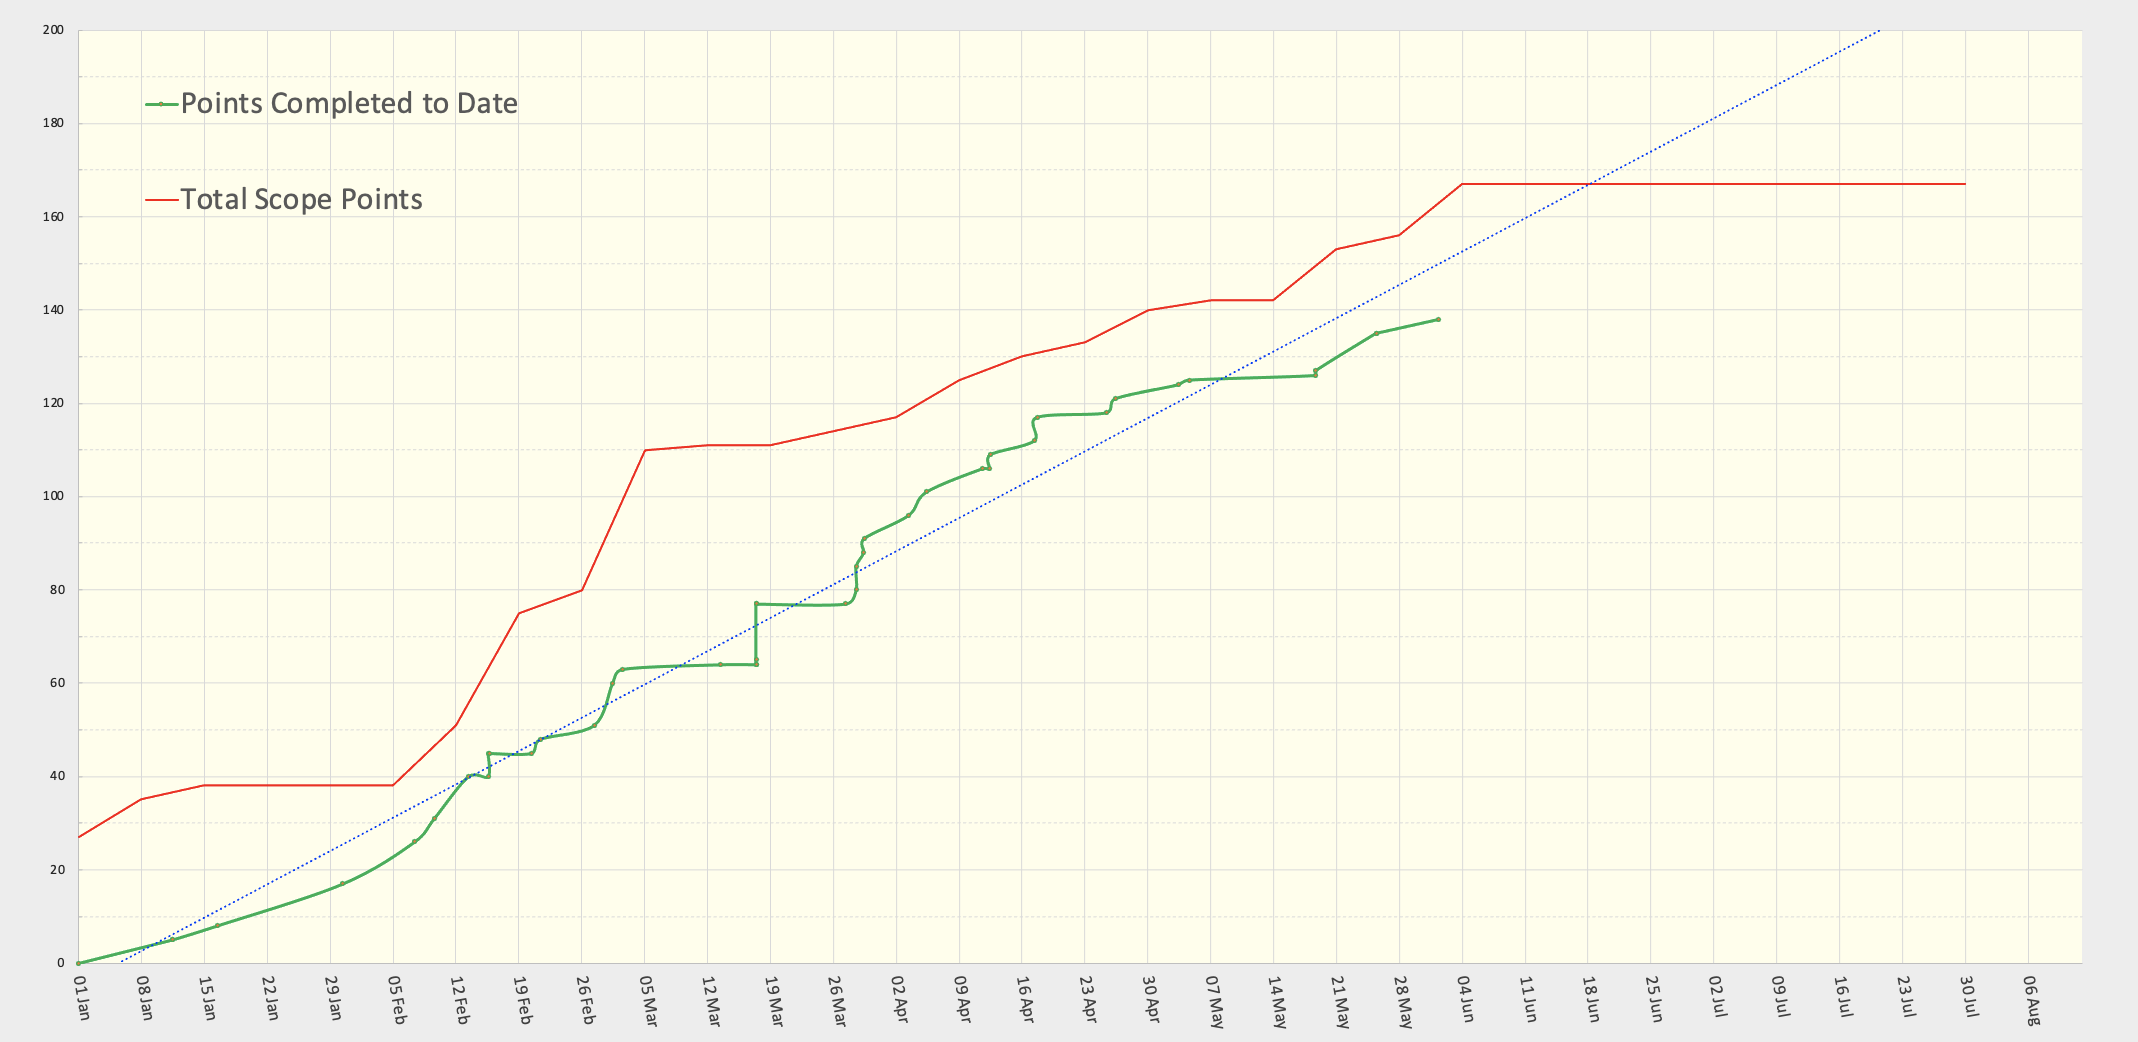
\includegraphics[width=6cm]{assets/burnup/2023-06-03.png}
    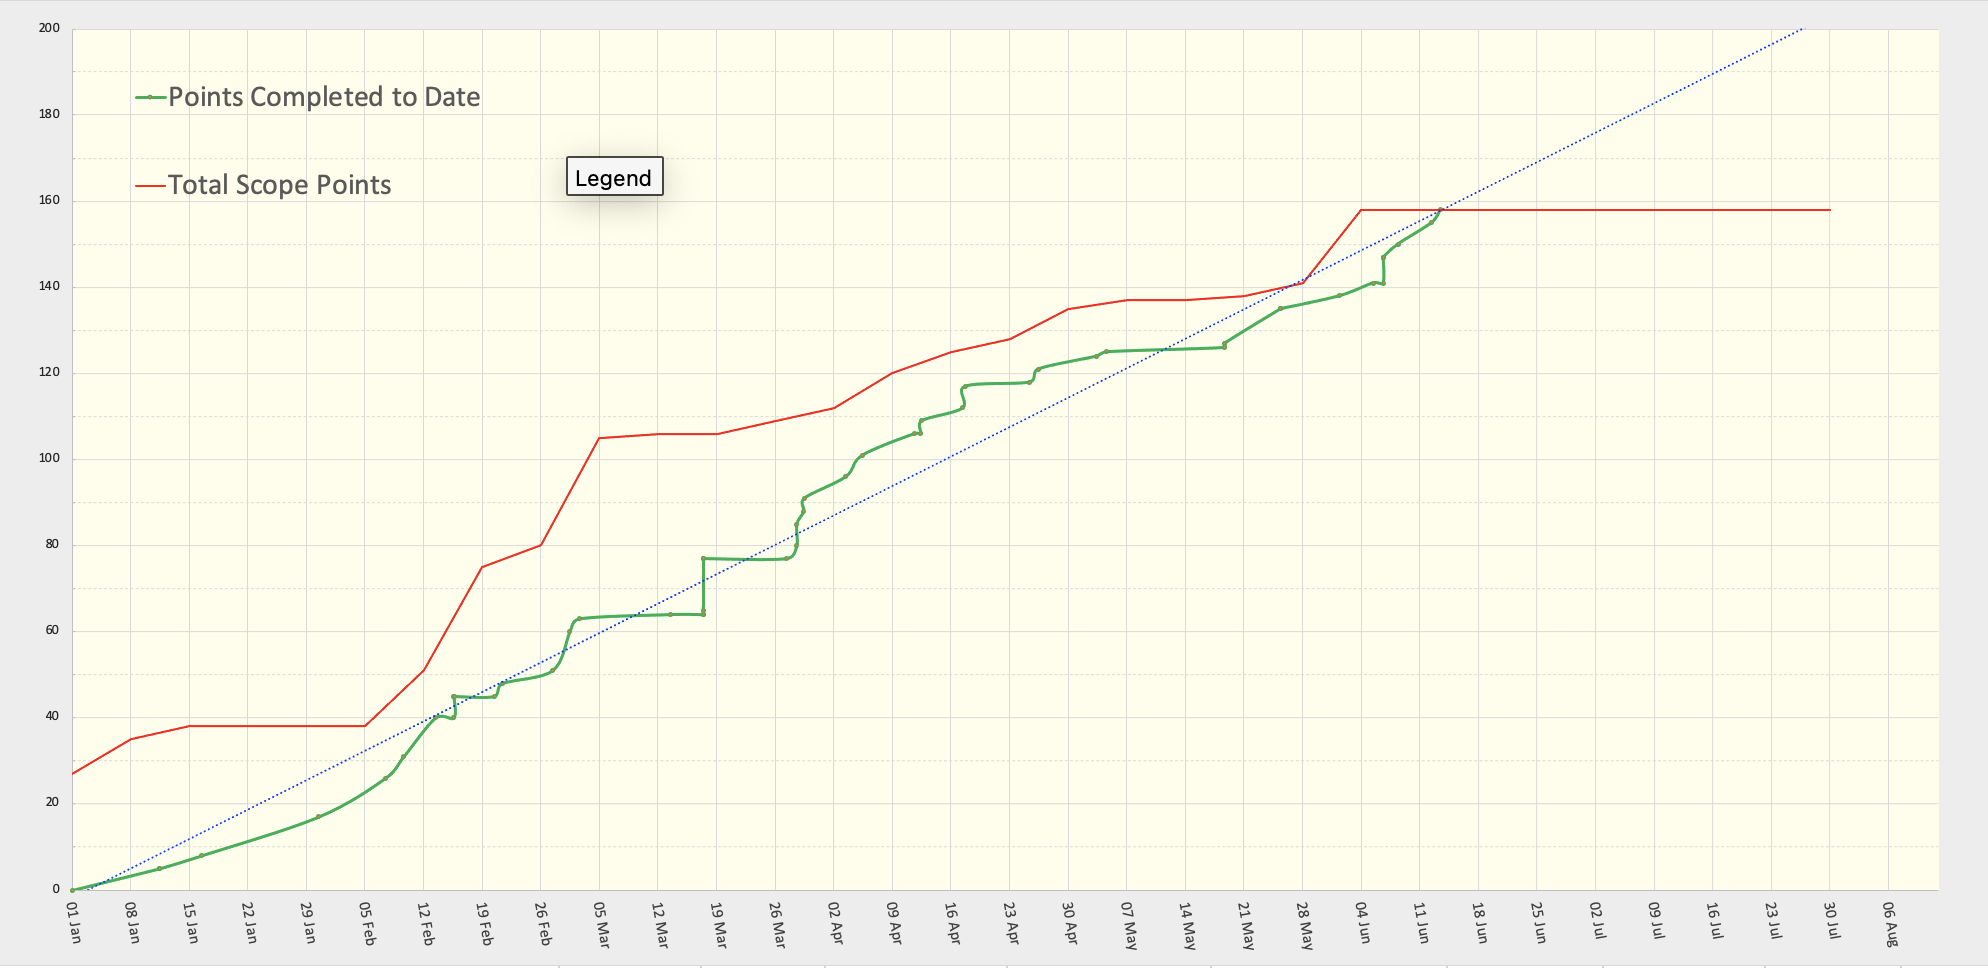
\includegraphics[width=6cm]{assets/burnup/2023-06-13.png}
    \caption{Exported graph of burn-ups overtime.}
    \label{fig:scheduleBurnup}
  \end{figure}

  The red line represents total amount of work todo, the dotted blue line is the expected projection of work completed overtime and the green line 
  is the amount of worked actually completed. As we discovered more work the we gradually got behind at first, however then began to get back 
  on track. Then scope creep, asks and deliverables [that] exceed the pre-set project scope [TODO2], kicked in as we added deltas to the MVP. As discussed 
  above this was then changed to come after and we were then able to finish on time.

  I found this helpful during the process as you could gauge where we were up to in the project. As well as the dropping of deltas on the MVP, automated 
  tests were picked up by devs, not just QA, which also helped us speed up development towards the end. I think these are great for time sensitive
  projects, however may add unneeded scrutiny and pressure on non time-sensitive projects.

  \subsection{Monitoring and issues}
  \todo[noline, size=\small]{L5}

  \subsection{Schedules deltas}
  \todo[noline, size=\small]{T1}
  As part of schedules \textit{'deltas'} were introduced, these deltas are notifications of changes to the underlying data. The end architecture looks
  like the below.

  \begin{figure}[H]
    \centering
    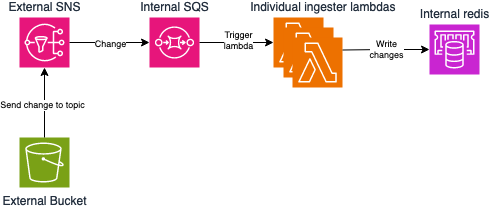
\includegraphics[width=10cm]{assets/scheduleDeltas.drawio.png}
    \caption{New delta architecture.}
    \label{fig:scheduleDeltas}
  \end{figure}

  The old method of having a control lambda run and fire off lambdas for each file is still present in the system, however this is now for maintenance
  only. The above allows us to get data to clients in real time, instead of being on a fixed timer for updating the data. We had a dev meeting where we 
  planned what to do and how to release it. We wanted to split the work up in a way that we would be able to release some of the work to live without
  affecting the current timer mechanism. This was tricky because as soon as the SQS was hooked up to trigger the lambda changes would be made to the data 
  potentially colliding with the coldstart.

  To fix this I suggested that we add a feature flag to \textit{'enable or disable functionality'} [TODO3], in the config that enables and disables writing 
  to redis. This would disable writing to redis on the LIVE environment and keep the event timer running to continue refreshing the later every 15 minutes.
  This would also allow us to write integration tests that run against the TEST and LIVE to make sure our deltas are working correctly and matching a full 
  restart.

  \begin{figure}[H]
    \centering
    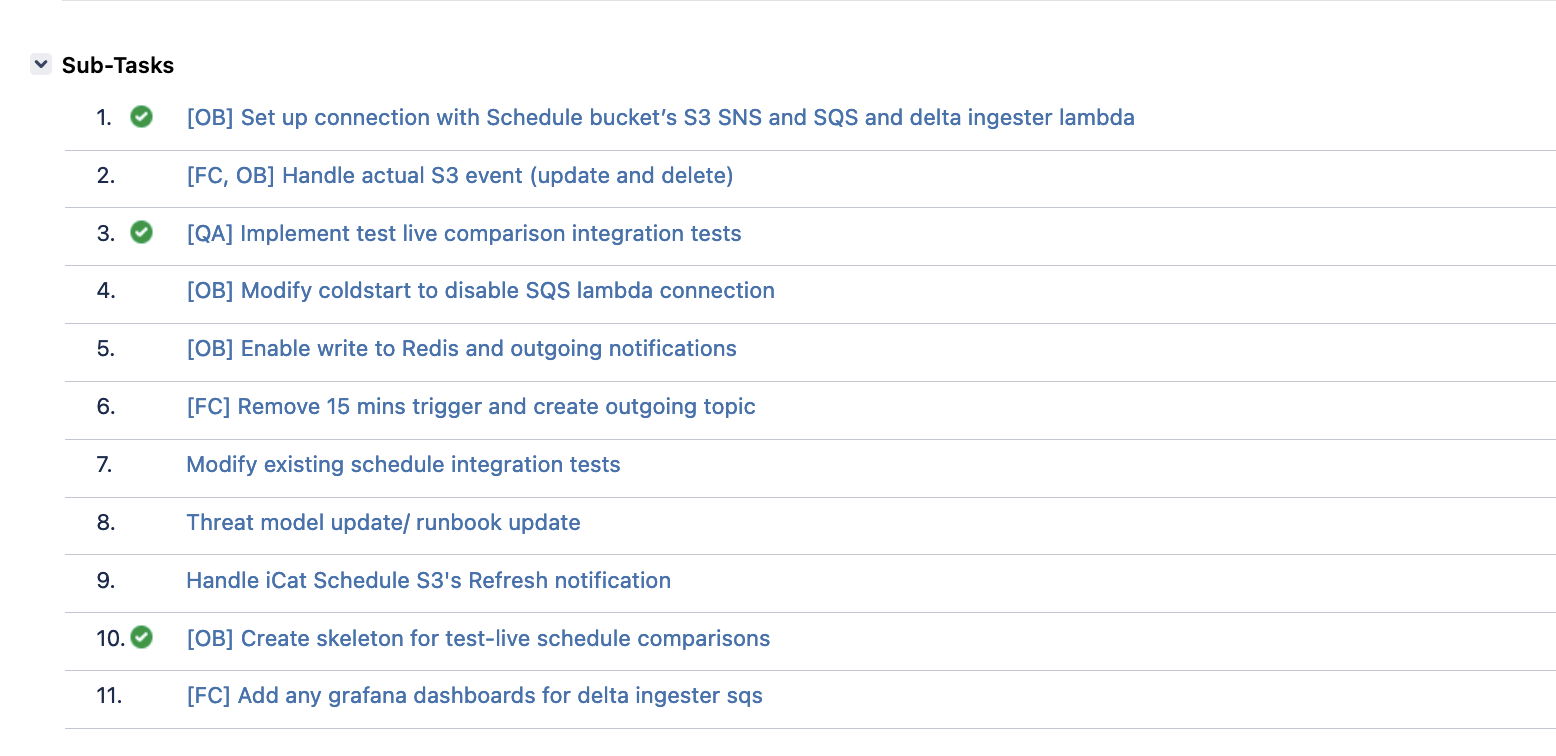
\includegraphics[width=10cm]{assets/scheduleDeltasTasks.png}
    \caption{Tasks to implement deltas into the ingester.}
    \label{fig:scheduleDeltasTasks}
  \end{figure}

  The above image highlights the tasks created to achieve implementing deltas. Using the above suggestion tasks 1, 2, 3 and 4 could all go to live,
  with tasks 5 and 6 being put on TEST to start deltas. Then the integration test can be ran to check the validity and gain confidence in the new 
  system. This keeps with the team aim for continuous deployment (CD) which allows \textit{'faster product development work [and] real-time feedback
  on new features, updates, and code changes'} [TODO4]. This allows us to quickly find issues with the system instead of deploying a large amount of 
  code all at once and it potentially failing in multiple places.

  \newpage
